\documentclass[12pt,oneside]{fithesis2}
\usepackage[english]{babel}       % Multilingual support
\usepackage[utf8]{inputenc}       % UTF-8 encoding
\usepackage[T1]{fontenc}          % T1 font encoding
\usepackage[                      % A sans serif font that blends well with Palatino
  scaled=0.86
]{berasans}
\usepackage[                      % A tt font if you do not like LM's tt
  scaled=1.03
]{inconsolata}
\usepackage[                      % Clickable links
  plainpages = false,               % We have multiple page numberings
  pdfpagelabels                     % Generate pdf page labels
]{hyperref}
\usepackage{titlesec}             % Allows creating custom \section's\usepackage{url}
\usepackage{blindtext}            % Lorem ipsum generator
\usepackage{listings}             % Code snippets
\usepackage{minted}               % Code snippets / assembly
    \usemintedstyle{bw}           % plain black higlighting
\usepackage{graphicx}
\usepackage{epigraph}
\usepackage{titling}
\graphicspath{ {img/} }

%% 
%\usepackage{background}
%\backgroundsetup{
%scale=1,
%angle=0,
%opacity=.4,  %% adjust
%contents={\includegraphics[width=\paperwidth,height=\paperheight]{pgfmanual}}
%}
%% 

% ------------------------------------------------------------------------------------------


%%%   End   %%%
\titleformat{\chapter}[display]
{\normalfont\huge\bfseries}{\chaptertitlename~\thechapter}{20pt}{\Huge}
\titlespacing*{\chapter}{0pt}{50pt}{40pt}
\titlespacing*{name=\chapter,numberless}{0pt}{-70pt}{10pt}
%%%   End   %%%


% ------------------------------------------------------------------------------------------


\thesislang{it}                   % The language of the thesis
\thesistitle{Analisi di Malware}       % The title of the thesis
\thesissubtitle{Reverse engineering di malware e realizzazione di una signature}  % The type of the thesis
\thesisstudent{Pape Alpha\hspace{3.5mm} Toure}          % Your name
%\thesiswoman{false}                % Your gender
\thesisfaculty{fi}                % Your faculty
\thesisyear{Esame di Stato \the\year}     % The academic term of your thesis defense
%\thesisadvisor{John Foo, Ph.D.}   % Your advisor


% this alters "before" spacing (the second length argument) to 0
%\titlespacing*{\chapter}{0pt}{0pt}{40pt}

% LINE SPACING
\renewcommand{\baselinestretch}{1.25}

% FOOTNOTE LINE LENGTH
\renewcommand{\footnoterule}{%
  \kern -3pt
  \hrule width 100mm %height 1pt
  \kern 2pt
}

%% FOOTNOTES %%
\setlength{\footnotesep}{\baselineskip}
%% FOOTNOTES %%

% PAR
\setlength{\parskip}{1em}


% QUOTE
\newcommand{\chapquote}[3]{\begin{quotation} \textit{#1} \end{quotation} \begin{flushright} - #2, \textit{#3}\end{flushright} }

% UNDERKINE CHAPTER HEADINGS
\titleformat{\chapter}
  {\normalfont\Large\bfseries}{\thechapter}{1em}{}[{\titlerule[0.4pt]}]

% FOOTNOTE
\renewcommand*{\thefootnote}{(\arabic{footnote})}

\begin{document}
  \FrontMatter                    % The front matter
    \ThesisTitlePage                % The title page
    %\begin{ThesisDeclaration}       % The declaration
    %  \DeclarationText
    %  \AdvisorName
    %\end{ThesisDeclaration}
    %\begin{ThesisThanks}            % The acknowledgements (optional)
    %  I would like to thank my supervisor\,\dots
    %\end{ThesisThanks}
    
    % blank page

%\setlength{\droptitle}{-4em}
%\addtolength{\droptitle}{-4pt}


\setlength{\droptitle}{-4em}   % This is your set screw

\newpage
\thispagestyle{empty}
\mbox{}

    
    \begin{ThesisAbstract}          % The abstract
      L’obiettivo del lavoro è quello di proporre una Signature, un insieme di regole identificative di software malevoli (malware) o loro\newline varianti. Il caso di studio prende in esame un banking trojan di nome Wirenet, un malware che si presenta all'utente come adattatore per Wi-Fi. Esso è dotato di numerose funzionalità che vanno dal furto di credenziali al controllo remoto della macchina infetta. Per analizzare Wirenet sono state utilizzate tecniche di reverse engineering.\newline Si pone attenzione sulle peculiarità riscontrate nella sua implementazione e su un possibile profilo degli autori. % \,\dots
    \end{ThesisAbstract}
    %\begin{ThesisKeyWords}          % The keywords
    %  keyword1, keyword2\,\dots
    %\end{ThesisKeyWords}
    

    \renewcommand\contentsname{Indice}
    \tableofcontents                % The table of contents
  
  \MainMatter                     % The main matter    
    \chapter*{Introduzione}
    \addcontentsline{toc}{chapter}{\protect\numberline{}Introduzione}
    
        % ------------------------------------------------------------------------------------------
        
        %\begin{figure}[h]
        %\centering
        %\includegraphics[width=\textwidth]{Figures/architecture.png}
        %\caption{Architettura del sistema}
        %\end{figure}
        
        % ------------------------------------------------------------------------------------------
        
        % QUOTE
        %\chapquote{``Begin at the beginning,¨ the King said gravely, ``and go on till you come to the end: then stop."}{Lewis Carroll}{Alice in Wonderland}
        
    
        \section*{Reverse Engineering}
        \addcontentsline{toc}{section}{\protect\numberline{}Reverse Engineering}
        L'ingegneria inversa (Reverse Engineering, da ora in poi \emph{RE}) è il processo che permette l'acquisizione di informazioni riguardo ad un\newline sistema, disassemblandolo ed analizzando le sue parti.
        Le sue modalità variano ampiamente in base al dominio entro cui 
        essa è applicata, ed agli obiettivi che si intendono raggiungere. Questi sono alcuni dei
        campi dell'informatica che vedono protagonista il RE:
        \setlength\labelsep   {\dimexpr\labelsep - 1.5em\relax}  
        %\setlength\leftmargini{\dimexpr\leftmargini + 0.5em\relax}
        \begin{itemize}
          \item \textbf{Interoperabiltà con software Legacy}: alcune aziende potrebbero avere la necessità di utilizzare software datato, la cui documentazione potrebbe non essere disponibile;
          \item \textbf{Formati di file proprietari}: lo sviluppo di alternative open source in grado di interpretare file dal formato proprietario, richiede una conoscenza della loro struttura;
          \item \textbf{Analisi di malware}: fornisce informazioni riguardanti funzionalità, vettori di attacco e metodi di contenimento;
          \item \textbf{Analisi di antivirus}: per ideare tecniche di elusione e verificare l'efficacia dei propri malware;
          \item \textbf{Algoritmi crittografici}: seppur sicuri teoricamente, le implementazioni di algoritmi crittografici possono presentare vulnerabilità.
        \end{itemize}
        %\clearpage
        \section*{I limiti dell'automazione nell'analisi di malware}
        \addcontentsline{toc}{section}{\protect\numberline{}I limiti dell'automazione nell' analisi di malware}
        % da Practical Malware Analysis
        %\subsection*{Sandbox}
        %\addcontentsline{toc}{subsection}{\protect\numberline{}Sandbox}
        Per automatizzare l'analisi di file vengono impiegate delle sandbox: dei meccanismi, cioè, di suddivisione dell'ambiente di esecuzione programmi. Le sandbox sono spesso utilizzate per ottenere rapidamente informazioni su file sconosciuti, ma non sono totalmente affidabili a causa dei seguenti limiti:
        %\setlength\labelsep   {\dimexpr\labelsep - 1.5em\relax}  
        %\setlength\leftmargini{\dimexpr\leftmargini + 0.5em\relax}
        \begin{itemize}
            \item Possono essere facilmente rilevate dai malware, i quali\newline modificherebbero i propri comportamenti o smetterebbero di funzionare del tutto. Apparentemente potrebbe sembrare una soluzione al problema ma, di fatto non lo è perchè impedisce all'analista di comprendere i meccanismi di funzionamento del malware;
            \item Non sono in grado di eseguire librerie che necessitano di file eseguibili da cui essere invocate;
            \item Non forniscono descrizioni approfondite delle funzionalità del malware;
            \item Non sono necessariamente in grado di fornire l'interazione necessaria per la corretta esecuzione del file;
            \item Sono lente e dispendiose e per questo vengono raramente adottate in soluzioni per utenti finali.
        \end{itemize}
        %Per 
        %\subsection*{Intrusion Detection Systems}
        %\addcontentsline{toc}{subsection}{\protect\numberline{}Intrusion Detection Systems}
        
        %Gli Intrusion Detection System sono software che monitorano la rete, in grado di rilevare attività sospette o malevole.
        %Gli IDS fanno uso di \emph{Network signatures}, firme identificative di malware caratterizzate dalle loro stesse caratteristiche a differenza di \emph{Host-based signatures} che analizzano le interazioni con il sistema operativo.
        
        %   E' OVVIO CHE DOBBIAMO ANCORA ANALIZZARLI MANUALMENTE
        %< E' ovvio >, una continua corsa che vede protagonisti nuovi malware e nuove firme per riconoscerli. Le Network signatures possono essere create attraverso tool automatici senza quindi dover analizzare manualmente a discapito della loro efficacia. 
        
        %A questo punto è chiaro che c'è ancora bisogno che qualcuno effettui analisi manuali.
        
        \clearpage
    % deduction and reversing
    \chapter*{Preparativi}
    \addcontentsline{toc}{chapter}{\protect\numberline{}Preparativi}
    Per questo studio è stato fatto uso di due macchine virtuali e software per analizzare in modo sicuro il malware.
    %Per maneggiare ed analizzare file di dubbia natura bisogna dotarsi dei giusti strumenti e delle giuste precauzioni. Ho quindi optato per una soluzione semplice da adottare e sufficientemente sicura. Ho quindi riutilizzato delle immagini di Windows in mio possesso usate precendentemente per reverse engineering e le ho riadattate perchè fossero sicure. La macchina su cui ho effettuato le analisi aveva il seguente setup:
    %\vspace{1.0mm}
    %\begin{itemize}
        %\item 
        
        \textbf{Windows 7}: Oltre ad eliminare accidentali esecuzioni, dispone di una versione Freeware di IDA, un disassembler, ovvero un programma in grado di tradurre il linguaggio macchina in codice assembly. E' lo standard di fatto più utilizzato tra i ricercatori di malware.
    %\end{itemize}
    \begin{center}
        \makebox[\textwidth]{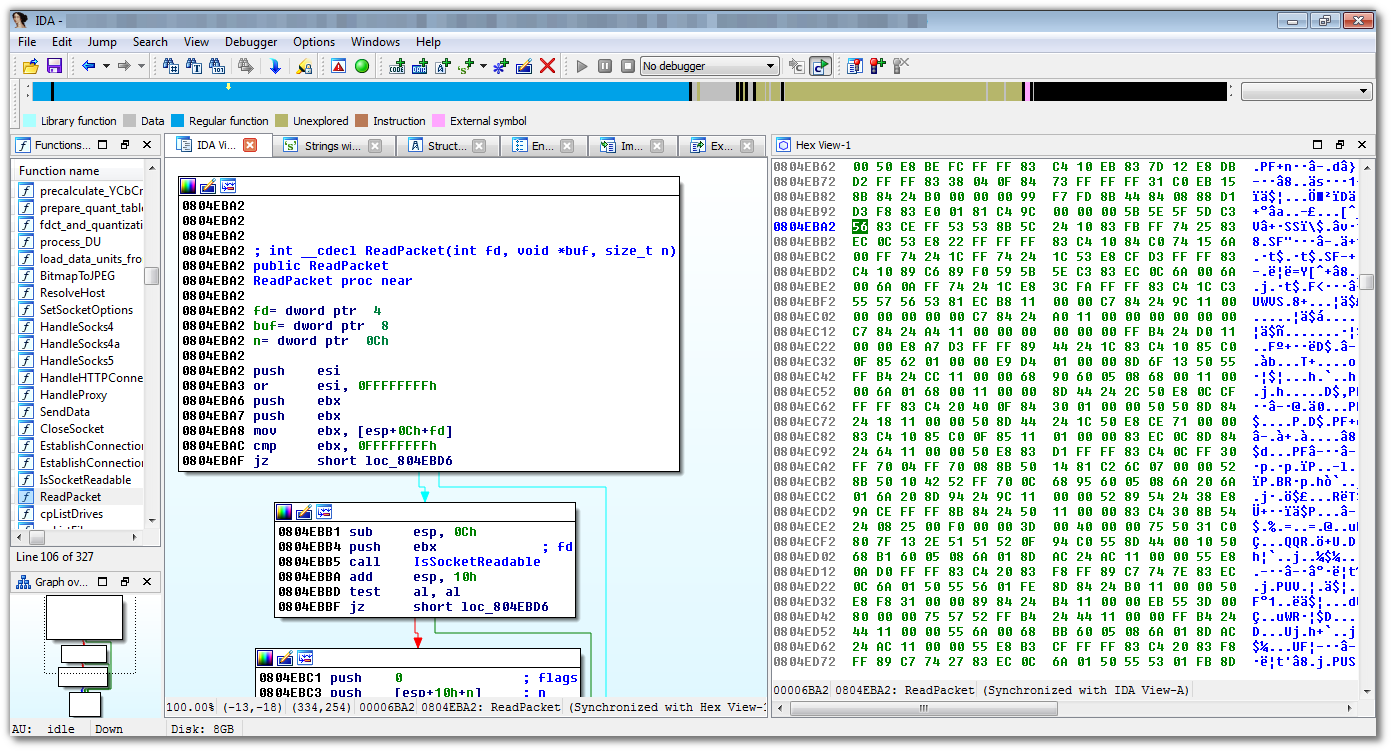
\includegraphics[width=\textwidth]{ida}} % 
    \end{center}
    %\begin{itemize}  
        %\item 
        \textbf{Ubuntu/Linux 14 LTS}: Questa macchina virtuale è stata dedicata prevalentemente ad analisi di tipo dinamico
            \begin{itemize}
                \item \textbf{Binwalk}: è strumento utilizzato prevalentemente per l'analisi ed il reverse engineering di immagini di firmware;
                \item \textbf{YARA}: è strumento in grado di analizzare e classificare file. Si possono creare descrizioni di famiglie di malware basate su pattern in comune.
     %       \end{itemize}            
    \end{itemize}
    \clearpage
    %Nel 2016 è stato attribuito ad un gruppo brasiliano "la colpa" di un banking trojan cross-platform. Lo scopo è quindi duplice: studio ed analisi delle funzionalità di malware ed
    %attraverso ad esso fare fronte a quella che può diventare la prossima frontiera dei malware (quelli cross-platform.
    %per questo ho analizzato questo sample più del 2012, per vedere se ci fossero riscontri tra i due casi)
    %
    \chapter*{Analisi del Malware}
    \addcontentsline{toc}{chapter}{\protect\numberline{}Analisi del Malware}
        %In questo capitolo viene descritto il nucleo del lavoro dell'analisi ed il processo di decompilazione        
        \section*{Vettori di infezione}
        \addcontentsline{toc}{section}{\protect\numberline{}Vettori di infezione}
        Del malware analizzato in questo studio non si è determinato con certezza il principale vettore di infezione nè il contesto in cui è stato utilizzato. Si suppone quindi che sia un malware \url{multistage}, che utilizza un archivio Java .jar (nome del file java.PDF.jar) per raccogliere informazioni riguardo all'host installare ed eseguire la corretta versione del malware.\newline Non avendo avuto alcuna possibilità di ottenere il dropper (cioè un programma creato per installare un malware su un sistema) si è cercato di ricostruire la prima fase del ciclo di vita del malware partendo dalle informazioni ottenute da un analisi comportamentale della sandbox di Virus Total.

        \begin{center}
            \makebox[\textwidth]{\includegraphics[width=\textwidth]{vt_jar}}
        \end{center}

        I nomi dei file, i loro tipi ed i rispettivi \url{hash} sono più che sufficienti per poter affermare con certezza che si tratta della payload della prima fase dell'attacco in quanto gli archivi Java quando aperti vengono automaticamente eseguiti. L'assenza della versione Linux del malware all'interno dell'archivio fa sorgere un dubbio in relazione alla provenienza sua infatti \url{Host1} e \url{Host2} sono le versioni Windows e OSX rispettivamente.\newline
        La ricostruzione del possibile attacco è basata sull'assenza dei seguenticomponenti fondamentali:\newline

        %\setlength\labelsep   {\dimexpr\labelsep - 1.5em\relax}  
        %\setlength\leftmargini{\dimexpr\leftmargini + 0.5em\relax}
        \begin{itemize}
            \item Meccanismi di autopropagazione
            \item Meccanismi di occultamento
            \item Exploit\footnote{Un exploit è un termine usato in informatica per identificare una tipologia di script che sfruttando una specifica vulnerabilità presente in un sistema informatico, permette l'esecuzione di codice malevolo su di esso con lo scopo di far ottenere all'attaccante l'acquisizione dei privilegi amministrativi.}
        \end{itemize}
        
        Di seguito sono illustrate due possibili dinamiche attraverso cui avvenivano le infezioni nel 2012:%\newline

        \textbf{Email}: sono ancora il vettore di attacco più efficace utilizzato dai criminali informatici. Lo \url{spear phishing} consiste in un attacco di ingegneria sociale\footnote{Nel campo della sicurezza informatica, l'ingegneria sociale è lo studio del comportamento individuale di una persona al fine di carpire informazioni utili.} mirato a specifici individui oppure ad organizzazioni. Esso si distingue dallo spam di email nel far largo uso di informazioni riguardanti i bersagli raccolte online per il successo dell'attacco. %Non essendo tante email non vengono cattate dai provider di email .%Non sono in grado di identificare con certezza il bersaglio di questo attacco. Diverse ragioni favoriscono aziende in favore di un pubblico aperto in primis i costi richiesti per condurre un attacco su larga scala:\newline 
        \vspace{1mm}
        
        \textbf{Exploit Kit}: un exploit kit è un insieme di programmi realizzati dai criminali per ovviare alla altrimenti lenta e complessa distribuzione di malware. Essi automatizzano il processo, individuando vulnerabilità nei client e sfruttandole per installare silenziosamente dei malware. Poichè exploit kit semplice può costare 500 dollari al mese, si ipotizza che gli autori del malware non ne avessero uno a disposizione. % Questa opzione non mi sembra viabile in quanto troppo avanzata e dispendiosa per il tipo di malware usato. Necessiterebbe di un architettura di rete di gran lunga più avanzata rispetto a quella utilizzata oppure di `cash` quasi sicuramente non a disposizione di questi tizi%\dots     % An exploit kit is a toolkit that automates the exploitation of client-side vulnerabilities, usually targeting browsers and programs that a website can invoke through the browser.
        \clearpage
        
        \section*{Installazione}
        \addcontentsline{toc}{section}{\protect\numberline{}Installazione}
        Dopo essere stato scaricato ed avviato sulla macchina vittima, Wirenet esegue le seguenti istruzioni:
        \begin{minted}[linenos]{nasm}
.text:0804CCE4 call    InitAESTables
.text:0804CCE9 lea     ebp, [esp+0C2Ch+var_C26]
.text:0804CCED call    InitTransfersList
.text:0804CCF2 call    ReadSettings
.text:0804CCF7 call    InstallPath
        \end{minted}
%[...]
%.text:0804CCE4 call    InitAESTables
%[...]
%.text:0804CCF2 call    ReadSettings
%.text:0804CCF7 call    InstallPath
%[...]        
        %Analizziamole più da vicino        
        %\setlength\labelsep   {\dimexpr\labelsep - 1.5em\relax}  
        %\setlength\leftmargini{\dimexpr\leftmargini + 0.5em\relax}
        %\begin{itemize}        
        %\item
        Si ponga l'attenzione sulle funzioni chiamate:
        
        \textbf{InitAESTables}: si limita ad inizializzare le P-BOX e le S-BOX dell'AES
        %\item
        \textbf{ReadSettings}: questa funzione recupera la configurazione default, composta da stringhe cifrate in RC4 all'interno del file stesso. Questo rende più complicata la scrittura di una firma che identifichi una famiglia malware in quanto le stesse informazioni, cifrate con chiavi diverse genererebbero risultati diversi.
        Questo non significa che le informazioni non possano però essere recuperate, in quanto la chiave è presente nel file. Utilizzando Binwalk si possono ottenere gli offset a cui si trovano le diverse sequenze di byte.
            
\begin{minted}{bash}
$ binwalk -R "\xc7\xd6\xac" wirenet

DECIMAL       HEXADECIMAL     DESCRIPTION
--------------------------------------------
62682         0xF4DA          \xc7\xd6\xac
\end{minted}            
            
            \clearpage
            
            Ripetendo la procedura per la chiave e tutte le stringhe contenute nella funzione \url{DecryptSettings}, si ottengono tutti gli ingredienti necessari per scrivere un programma in grado di decifrare le stringhe e restituire quanto segue
                \begin{minted}
                {bash}
$ python src/decode_settings.py wirenet
ConnectionString: 212.7.208.65:4141;
ProxyString: -
Password: sm0k4s523syst3m523
HostId: LINUX
MutexName: vJEewiWD
InstallPath: %home%/WIFIADAPT
StartupKeyName1: WIFIADAPTER
StartupKeyName2: -
KeyLoggerFileName: %Home%\.m8d.dat
BoolSettingsByte: 237
ConnectionType: 001
                \end{minted}
                
            % \clearpage
            %\vspace{2.5mm}
            %\item 
            \textbf{InstallPath}: La funzione attraverso /proc\footnote{Nei sistemi operativi Unix-like procfs è uno pseudo-filesystem usato per accedere alle informazioni relative ai processi fornite dal kernel. Il filesystem si trova solitamente montato nella directory /proc; poiché non è un filesystem reale, esso non occupa spazio sul disco rigido ed una limitata quantità di memoria.} ottiene il percoso a Wirenet si copia in \url{\~/WIFIADAPT} e si esegue. Per garantire una persistenza sul sistema, viene creato un file \url{\~/.config/autostart.desktop} per avviare il malware all'avvio del sistema.
            \begin{minted}{text}
[Desktop Entry]
Type=Application
Exec=%s
Hidden=false
Name=%s
            \end{minted}
            E' stato correttamente previsto il caso in cui non fossero installati Desktop Environments e che quindi il file di configurazione appena illustrato non venisse utilizzato. Si è ovviato inserendo nel file \url{\~/.xinitrc} un comando apposito, eseguito all'avvio del server X dal programma \url{xinit}.
            \begin{minted}{bash}
filename&
            \end{minted}
            L'aggiunta di un '\&' avvia il programma in background.
            
            Si rilevano due grandi mancanze: l'aver eliminato la prima versione del file approdata sul sistema e la mancata gestione dei segnali ricevuti dal programma. Mirai\footnote{Mirai è un malware che trasforma i sistemi informatici in botnet controllabili da remoto, le quali possono essere utilizzate in attacchi informatici su larga scala.} ha correttamente affrontato entrambe le problematiche
            \begin{minted}[linenos]{c}
unlink(args[0]);
[...]          
            \end{minted}            
            La prima istruzione ad essere eseguita è un \url{unlink} che permette di eliminare il file di nome specificato come argomento di funzione, in questo caso se stesso. La persistenza fisica dei file su disco rende molto più semplice il lavoro dei ricercatori, in quanto fintantochè non si riesce ad ottenere una versione del malware non lo si può analizzare per creare firme.
        
            Si osservi ancora una volta la premura che Mirai dedica nel impedire che qualunque altro programma interferisca con se stesso
            \begin{minted}[linenos]{c}
// Signal based control flow
sigemptyset(&sigs);
sigaddset(&sigs, SIGINT);
sigprocmask(SIG_BLOCK, &sigs, NULL);
signal(SIGCHLD, SIG_IGN);
signal(SIGTRAP, &anti_gdb_entry);                     
            \end{minted}
            La chiamata \url{signal()} assegna ad un segnale, uno specifico handler. Questo permette ad ogni programma di ridefinire i propri comportamenti in risposta a specifici segnali. \url{SIGTRAP} è il segnale utilizzato da un processo per poter fermare l'esecuzione di un altro.\newline In sistemi UNIX la chiamata di sistema \url{ptrace()} permette ad un processo di controllarne un altro, costituendo quindi la base di tutti i debugger.  Più specificatamente, in architetture che supportano\newline breakpoints, nel momento in cui la CPU esegue un'istruzione che genera un interrupt, l'esecuzione viene affidata all'handler corrispondente nel IDT\footnote{La Interrupt Descriptor Table (IDT) è una struttura dati usata dalle architetture x86 per implementare una tabella di vettori interrupt. La IDT è usata dal processore per determinare la corretta risposta a interrupt e eccezioni.}.
            Nel momento in cui la CPU riceve un interrupt, essa passa in kernel-mode ed infine notifica il debugger del breakpoint raggiunto dal programma debuggato.            
        %\end{itemize}   
        \clearpage

        Durante l'esecuzione di \url{InstallHost} oltre all'opzione di essere eseguito come demone, ne segue una caratteristica dei banking trojan, ovvero un keylogger
        
        \begin{minted}[linenos]{nasm}        
.text:08052D95 push    esi
.text:08052D96 push    esi
.text:08052D97 push    0               ; arg
.text:08052D99 push    offset cpStartKeyLogger ; start_routine
.text:08052D9E call    cpBeginThread
        \end{minted}

        %Il keylogger in questione utilizza <api di cui non ricordo il nome> messe a disposizione da Linux per intercettare e registrare i vari eventi.
        
        %Quelli più interessanti sono quelli riguardanti la tastiera.
        %E' qui in seguito mostrata lo pseudo codice relativo all'hooking degli eventi
        
        \section*{Keylogger}
        \addcontentsline{toc}{section}{\protect\numberline{}Keylogger}        
        Il keylogger utilizza \url{XOpenDisplay()} per connettersi al server X
        \footnote{X Window System è un gestore grafico, standard de-facto per molti sistemi Unix-like.}
        del sistema, dopo di che usa \url{XQueryExtension()} per sapere se l'estensione del protocollo X che gestisce gli input è presente \url{("XInputExtension")}. Con questo ultimo handle all'estensione, sfrutta \url{XListInputDevices} per ottenere la lista dei dispositivi connessi ricercandone due specifici di nome \url{System keyboard} e \url{AT}. A questo punto con \url{XOpenDevice()} si apre il dispositivo appena individuato e si selezionano gli eventi da intercettare con \url{XSelectExtensionEvent()}. Da da questo momento in poi, tutti i tasti premuti vengono salvati nel file \url{\~/.m8d.dat}.\newline Ricostruendo le strutture dati utilizzate si decompila parte del keylogger nel seguente modo:\clearpage
\begin{minted}[linenos]{c}
XKeyEvent *hooks;

[...]

while (TRUE) {
    // Gets an event from the 'XEvent' queue
    // Intercept the event
    XNextEvent (&display, &single_event);
    
    // Acquire its information
    hooks.type = single_event.type;
    hooks.display = single_event.xcreatewindow.display;
    hooks.root = single_event.xproperty.time;
    hooks.time = single_event.xkeymap.key_vector[12];
    hooks.y = single_event.pad[10]
    hooks.y_root = single_event.pad[12]
    hooks.keycode = single_event.pad[14]
    
    // Save it to a file
    LogKey (hooks, hooks, &display);
}

XCloseDisplay ();
[...]
\end{minted}

    %Riconoscere questo tipo di keylogger non è complicato poichè è parte di un processo user-space ed in quanto tale non è in grado di agire ad un livello abbastanza basso come quello di un driver kernel-mode. 
    Il codice del keylogger viene eseguito all'interno di un processo user-space, un processo che non appartiene al sistema operativo. I keylogger in kernel-space possono essere implementati come driver che registrano gli eventi ed in quanto tali possono facilmente bypassare analisi di applicazione in user-space. %Nonostante la sua semplicità, esso rappresenta una minaccia Windows per anni non è che si siano inventati stregonerie.
        \clearpage

        \section*{Architettura}
        \addcontentsline{toc}{section}{\protect\numberline{}Architettura}
        %\subsection*{Command and control}
        %\addcontentsline{toc}{subsection}{\protect\numberline{}Command and control}
        L'architettura di rete è molto semplice: gli host infetti stabiliscono una connessione con il server di controllo detto Command and Control (C\&C), eventualmente attraverso server SOCKS\footnote{Un server SOCKS è un particolare tipo di proxy che permette di effettuare connessioni TCP dirette (e, dalla versione 5, di veicolare traffico UDP oltre che TCP) tra computer su due reti IP differenti nei casi in cui un instradamento diretto (routing) non sia disponibile} aperti da altre macchine infette.\newline
        Wirenet invia un pacchetto contenente \url{RGI28DQ30QB8Q1F7}, una stringa di autenticazione. Le comunicazioni vengono rese sicure tramite un implementazione dell' AES in modalità CFB\footnote{In crittografia la modalità di funzionamento dei cifrari a blocchi è una serie di procedimenti standard di un algoritmo che operi tramite cifratura a blocchi per garantire la sicurezza di testi o messaggi di lunghezza a piacere.} utilizzando \url{sm0k4s523syst3m523} come password. I dettagli specifici riguardanti le modalità di funzionamento dei cifrari a blocchi non sono utili ai fini di questo lavoro e per tale ragione sono stati omessi. Dopo la generazione di numeri casuali viene cifrato la stringa di autenticazione        \begin{minted}{nasm}
.text:08054B02 push    offset TestPacket
.text:08054B07 push    offset InitializationVector
.text:08054B0C push    10h
.text:08054B0E push    1
.text:08054B10 push    eax
.text:08054B11 call    AESCryptCFB
        \end{minted}
        \clearpage
        
        %\begin{wrapfigure}{r}{0.25\textwidth} %this figure will be at the right
        %    \centering
        %    \includegraphics[width=0.25\textwidth]{SendAuthenticationPacket2}
        %\end{wrapfigure}
        In caso \url{AESCryptCFB} avvenga con successo, viene utilizzata \url{SendData} per trasmettere i dati cifrati al server C\&C
        \begin{center}
            \makebox[\textwidth]{\includegraphics[width=\textwidth]{SendAuthenticationPacket2}} %
        \end{center}
        %\subsection*{Crittografia Asimmetrica}
        %\addcontentsline{toc}{subsection}{\protect\numberline{}RSA and asymmetric crypto}
        %WannaCry è un ransomware\footnote{Un ransomware è un tipo di malware che limita l'accesso del dispositivo che infetta, ne cifra i file e richiede un riscatto per ripristinare l'accesso al computer.} che ha infettato più di 400,000 computer, alcuni appartenenti ad ospedali ed università. I ransomware operano creando chiavi simmetriche casuali utilizzate per la cifratura dei file della vittima, trasmettono queste chiavi in modo sicuro cifrandoli con la chiave pubblica del server C\&C e le distruggono. La combinazione più diffusa è composta dall'AES e dall'RSA.        
        %\clearpage        
        La dispendiosa analisi dell'AES non ha prodotto risultati poiché\newline l'implementazione non presenta bug rilevanti sfruttabili per un exploit. L'utilizzo di un timestamp per generare gli Initialization Vectors ovvero i numeri pseudo-casuali utilizzati dal Cipher Feedback, viola uno dei requisiti richiesti per mantenere l'integrità del CFB ovvero la non prevedibilità del IV. Lo studio delle implementazioni degli algoritmi crittografici trova una più ampia applicazione nei ransomware, per trovare modi di recuperare file cifrati.   
        %\vspace{2.5mm}
        \clearpage
        Dopo aver controllato che la dimensione dei pacchetti ricevuti e il tipo siano validi viene invocato l'handler dei comandi, il nucleo del malware
        
        \begin{minted}[linenos]{nasm}        
.text:0804CDAA dec     ebx
.text:0804CDAB push    ebx             ; int
.text:0804CDAC lea     eax, [esp+0C30h+filename]
.text:0804CDB0 push    eax             ; filename
.text:0804CDB1 push    edi             ; int
.text:0804CDB2 push    esi             ; arg
.text:0804CDB3 call    ProcessData
        \end{minted}
        
        Questa funzione (\url{ProcessData}) è una delle più grandi all'interno del file. E' composta da uno switch case in grado di gestire 64 diverse casi, ognuna delle quali corrisponde ad una funzioni del malware.
        
        %A differenza le versioni per OSX e Windows, questo file seppure strippato\footnote{Un file binario senza informazioni di debug avendo quindi una dimensione minore} ha mantenunto informazioni di debug, quali i nomi delle funzioni.
        
        \clearpage
        
        
        
        %\subsection*{Controllo remoto}
        %\addcontentsline{toc}{subsection}{\protect\numberline{}Controllo remoto}
        
        %Ho buttato qui alcune tra le funzionalità più interessanti (39 dedicate al controllo remoto)
        
        
        %\textbf{cpMouse*}: Queste funzioni permettono di controllare il mouse della macchina infetta dal server Command and Control
        
        %\textbf{cpScreenCapture}: Questa funzione è sorprendente per via dell'impegno preso dagli autori di implementare da zero. (Fa uno screenshot, lo converte da bitmap a JPEG e poi lo manda)
        %Per ragioni riguardanti la sua importanza all'interno del malware e della sua complessità mi limiterò ad un overview ad alto livello:
        
        
        \section*{Applicazioni bersagliate}
        \addcontentsline{toc}{section}{\protect\numberline{}Applicazioni bersagliate}
        %The malware is designed to target a wide variety of applications that are 
        %likely
        %to be present. Older Mozilla products (i.e. Firefox 3.5 - 32.0), handle login 
        %credentials
        %storage in the same way, by having an encrypted database storing the file 
        %\textit{key3.db}. 
        %order to access the data, it is first necessary to know 
        %all the available profiles for any given Linux user on the computer.
        %As such, after iterating through all the files in \textit{/usr/lib} looking 
        %for
        %folders satisfying the following regular expression \textit{firefox-3*, 
        %firefox-4*, thunderbird-*}, \textit{libmozsqlite3.so} is loaded.
        %Mozilla products use Network Security Services, a set of libraries designed to develop security enhanced applications. 
        %Attackers can steal credentials 
        %pretty trivially, by leveraging the same exact procedure used by legitimate
        %programs and handing them over to the Command and Control server.
        %There's not way to detect whether a master password is set and there is no handling of that case.
        %The decompiled functions looks as follows:        
        
        Il malware è stato progettato per rubare le credenziali utilizzate in una grande varietà di prodotti, tutti comunemente utilizzati come browser e client per email. I prodotti Mozilla condividono lo stesso meccanismo per salvare email e password: utilizzano un database SQLite criptato di nome \url{key3.db}. Per ottenere i dati utilizzati in \newline Firefox per esempio, è necessario conoscere i vari profili presenti, e ripetere il processo di estrazione per ognuno di essi. Tramite espressioni regolari \url{firefox-3*}, \url{firefox-4*}, \url{thunderbird-*} vengono cercate in \url{/usr/lib} le cartelle contenenti le rispettive librerie necessarie per l'interazione con il database a seconda del servizio. Firefox, Thunderbird e Seamonkey usano \url{Network Security Services}, un insieme di librerie in grado di fornire servizi crittografici. Dopo aver caricato le librerie necessarie, si è in grado di accedere alle credenziali normalmente sfruttando la stessa identica procedura utilizzata da programmi legittimi. Non viene però gestito il caso in cui un profilo adotti una master password, ovvero una password con cui vengono cifrate tutte le credenziali. La query al database viene decompilata come segue:
        
        \begin{minted}[linenos]{c}
// Connect to the database
sqlite3_open("...", db_handle);

// Prepare the SQL statement
sqlite3_prepare_v2 (database, 
                    "select *  from moz_logins", 
                    25, 
                    stmt,
                    ...);
// Initialize a NSS object
NSS_Init (...);

// Get a Slot ID, just an ID
keySlot = PK11_GetInternalKeySlot ();

PK11_Authenticate (keySlot);

// Get the return values of the previous query
sqlite3_column_text (stmt, ...);

// Data is base64encoded
NSSBase64_DecodeBuffer ();

// A blank password is used if no master password is set
PK11SDR_Decrypt ();

// See if the query was executed successfully
sqlite3_step ();
        \end{minted}
        
Oltre a Thunderbird, Firefox, e SeaMonkey le seguenti applicazioni sono vulnerabili ad un attacco simile a quello appena illustrato
\begin{itemize}
    \item Opera
    \item Google Chrome
    \item Google Chromium
    \item Pidgin
\end{itemize}
        
        
        \clearpage
        
        \section*{Remote Administration Tools}
        \addcontentsline{toc}{section}{\protect\numberline{}Remote Administration Tools}
        %Unlike traditional banking trojans, wirenet feature extensive remote administration functionalities. First and foremost there's the classic reverse bind shell: the malware spawns a shell, duplicates file descriptors and connects back to the Command and Control server. 
        %This results in the attackers having a fully working shell into the system without having to deal with the hassle of opening a local port and attempting to establish a connection going through firewalls.
        %Moreover, it is capable of inspecting disks, downloading, deleting, renaming and everything that can be done with files. On top of this common functionalities among malware and remote exploits, there are extensive capabilities that go as far as controlling mouse, renaming windows and taking screenshots.
        %They all use native Linux API to interact with devices connected to the computer.
        A differenza dei classici banking trojan gli autori di Wirenet hanno investito notevolmente nell'implementazione di funzionalità atte alla sorveglianza dell'utente come il controllo del mouse, delle finestre e catture dello schermo. Non sono state tralasciate funzionalità di amministrazione remota come la navigazione nei drive, i download, la rimozione di file e la terminazione dei processi. % Oltre a queste comuni funzionalità caratteristiche dei malware e degli exploit remoti, ci sono         
        In fine è presente una classica reverse bind shell: una shell locale i cui descrittori di file vengono duplicati ed assegnati al socket su cui è in corso la comunicazione. Questa procedura permette di fornire terminali agli host della rete anche attraverso eventuali firewall.
        \begin{center}
            \makebox[\textwidth]{\includegraphics[width=\textwidth, height=3cm]{reverse_bind_shell.png}}
        \end{center}
        \clearpage
        \section*{George Orwell on Surveillance}
        \addcontentsline{toc}{section}{\protect\numberline{}George Orwell on Surveillance}
        \chapquote{"Those who do not move, do not notice their chains."}{Rosa Luxemburg}{}
        George Orwell's 1984  showcases the life of Winston, a men living in a country ruled by a totalitarian government. The Party, the name of the government ruled by a mysterious figure called Big Brother, truly stretches the meaning of totalitarism because of the means by which it controls people. It does so by employing a wide variety of methods most notably the constant audio video surveillance of people's houses. Moreover, it makes use of an authority called Thought Police entitled of finding anyone who commits a Thoughtcrime, namely an illegal thought. On top of using an aggressive propaganda and actively destroying citizens' critcal thinking skills, the Party has adopted Newspeak: a simplified version of English that removes concepts entirely, thus making certain thoughts impossible.\par Edward Snowden leaked classified NSA documents, disclosing multiple global surveillance programs run by NSA and the Five Eyes Intelligence Alliance. The threat Orwell was warning us about has already striken: global surveillance programs like PRISM, XKeyScore have gone far beyond their initial scope, national security. The evergreen argument "I have nothing to hide" which is never supported by actions, delivers multiple fallacious believes one of them is that only bad people have things to hide, consequentially making us only more and more willing to be compliant to whatever expectation has to be met. As Orwell showed, privacy has never been a matter of hiding malicious things, as it has always been about freedom. 
        
        \chapter*{Signature-Based Detection con YARA}
        \addcontentsline{toc}{chapter}{\protect\numberline{}Signature-Based Detection in YARA}
        \begin{center}
            \makebox[\textwidth]{\includegraphics[width=\textwidth, height=3cm]{yara.png}}
        \end{center}
        \chapquote{ The pattern matching swiss knife for malware researchers (and everyone else)}{Virus Total}{Documentation}
        
        Yara è un programma utilizzato principalmente nell'analisi di \newline malware nel loro rilevamento. Utilizza un approccio basato su regole che descrivono famiglie di malware. Ogni regola consiste in un pattern testuale oppure binario da ricercare all'interno del file.\newline
        Si considerino le seguenti istruzioni e si cerchi di scrivere una regola in Yara per identificarle.
        
        \begin{minted}[linenos]{nasm}
                sub_100012BC proc near
0F 20 C0        mov     eax, cr0
25 FF FF FE FF  and     eax, 0FFFEFFFFh
0F 22 C0        mov     cr0, eax
C3              retn
                sub_100012BC endp
        \end{minted}
        
        Nell'architettura x86 il registro CR0 contiene diversi flag che\newline modificano il comportamento della CPU quali la paginazione, la cache e la modalità protetta. Il bit più interessante è il 16esimo che, se non settato, permette la scrittura su pagine normalmente read-only. Questo è un componente chiave per i rootkit\footnote{Il rootkit è una collezione di software che si preoccupano di mascherare sé stessi o altri programmi.} che hanno bisogno di applicare modifiche al sistema operativo perchè rimangano nascosti.
        
        Di seguito si descrive una regola che segnala tutti i file che presentano le stringhe corrispondenti alle operazioni che interagiscono con elementi critici del sistema: x86\_rootkit
        
        \begin{minted}[linenos]{text}
rule x86_rootkit {

    strings:
        $rk1 = { 0F 20 C0 }       // mov     eax, cr0
        $rk2 = { 25 FF FF FE FF } // and     eax, 0FFFEFFFFh
        $rk3 = { 0F 22 C0 }       // mov     cr0, eax
        
    condition:
        all of them
}
        \end{minted}
        %Per capire la qualità richiesta perchè la firma migliori il detection rate ho fatto affidamento ancora una volta ai servizi di Virus Total che a loro volta fanno uso di API di rispettivi av vendor.
        Per scrivere una buona regola bisogna considerare gli aspetti più difficili da cambiare tra varianti. Il denominatore comune tra i banking trojan è la mappatura dei tasti tipica di keylogger necessaria a salvare su file i vari tasti premuti, un'altra caratteristica comune sono i percorsi dei file appartenenti alle varie applicazioni sulle varie\newline piattaforme.
        
        % Windows
        %
        %   Firefox: %APPDATA%\Mozilla\Firefox
        %   Thunderbird: %APPDATA%\Thunderbird
        %   SeaMonkey 2.0+: %APPDATA%\Mozilla\SeaMonkey.
        %
        % OSX
        %
        %   Old Opera: C:\users\<username>\AppData\Roaming\Opera\Opera\profile\wand.dat Opera 16.0
        %   New Opera: C:\Users\user_name\AppData\Roaming\Opera Software\Opera Stable\

    \chapter*{Conclusioni}
    \addcontentsline{toc}{chapter}{\protect\numberline{}Conclusioni}        
        \section*{L'ultima fase}
        \addcontentsline{toc}{section}{\protect\numberline{}L'ultima fase}
        L'ultima ma non meno importante fase del progetto consiste nel rendere disponibile l'analisi effettuata agli sviluppatori di antivirus, in modo che quest'ultimi possano integrare i propri software con il gli elementi necessari per riconoscere le varianti di questo malware. WannaCry è un ransomware\footnote{Un ransomware è un tipo di malware che limita l'accesso del dispositivo che infetta, ne cifra i file e richiede un riscatto per ripristinare l'accesso al computer.} che ha infettato più di 400.000 computer grazie ad ETERNALBLUE, un exploit del NSA che sfrutta una vulne-\newline rabilità per cui Microsoft aveva rilasciato una patch due mesi prima, dimostrando che non è sufficiente migliorare misure di sicurezza se queste poi non vengono adottate. Sono ancora numerosi gli Antivirus non in grado di riconoscere Wirenet, sono 14 secondo le API Virus Total tra cui alcuni di alta qualità come Malwarebytes.
        \section*{Pubblicazione del lavoro}
        \addcontentsline{toc}{section}{\protect\numberline{}Pubblicazione del lavoro}
        Il codice decompilato di Wirenet, il file utilizzato, la signature in YARA e questo documento sono disponibili su GitHub sotto la licenza BSD-2 all'indirizzo seguente
        \begin{itemize}
            \vspace{-1.25em}
            \item \url{https://github.com/shxdow/wirenet-analysis} 
        \end{itemize}
        \vspace{-1.25em}
        La versione di Wirenet si può identificare con i seguenti hash
        \begin{itemize}
            \vspace{-1.25em}
            \item MD5 \url{9A0E765EECC5433AF3DC726206ECC56E}
            \item SHA1 \url{5996d02c142588b6c1ed850e461845458bd94d17}
        \end{itemize}
        
    % A list of books / resources used
    \setlength\labelsep   {\dimexpr\labelsep + 1.5em\relax} 
    \renewcommand\bibname{Bibliografia}
    % not sure what that '9' is for, but shit "just breaks".
    \begin{thebibliography}{10}
    \bibitem{Practical RE} 
    Bruce Dang and Alexandre Gazet.
    \textit{Practical Reverse Engineering: x86, x64, ARM, Windows Kernel, Reversing Tools, and Obfuscation} Feb 17, 2014
 
    \bibitem{Practical Malware Analysis} 
    Michael Sikorski and Andrew Honig.
    \textit{Practical Malware Analysis: The Hands-On Guide to Dissecting Malicious Software by Michael Sikorski and Andrew Honig } Mar 3, 2012
    
    \bibitem{Practical Malware Analysis} 
    Ryan elfmaster O'Neill.
    \textit{ Learning Linux Binary Analysis } Feb, 2016

    \bibitem{Yurichev RE} 
    Dennis Yurichev.
    \textit{ Reverse Engineering for Beginners }

    \bibitem{Linux Kernel} 
    Robert Love.
    \textit{ Linux Kernel Development (3rd Edition) } Jul 2, 2010
    
    \bibitem{IDA Book} 
    Chris Eagle.
    \textit{ The IDA Pro Book 2nd edition } Jul, 2011

    \bibitem{Orwell} 
    George Orwell.
    \textit{ 1984 } Jun 8, 1949
    
    \end{thebibliography}
\end{document}
